\documentclass{beamer}
\usepackage{setspace}
\usepackage{bm,color,float,epstopdf,amsthm,epstopdf}
\usepackage{multirow}
\newtheorem{result}{Result}
%\title{\large Financial Options}
%\author{FNCE 3010: Corporate Finance}
\begin{document}
%\maketitle

\begin{frame}{Options}
    \begin{center}
        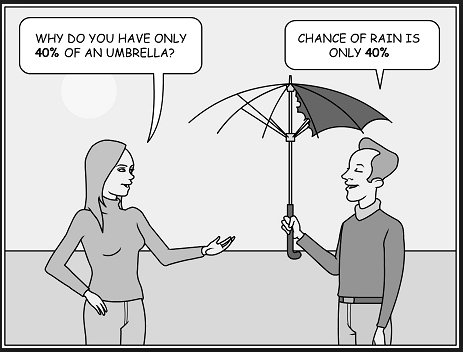
\includegraphics[scale=.5]{umbrella}
    \end{center}
\end{frame}

% Financial Options
\begin{frame}{Overview}
\begin{itemize}
\item Financial options are one of the most important and actively traded financial assets and important tools for corporate financial managers. 
\item We can think of the capitalization of the firm itself---that is, its mix of debt and equity---as options on the underlying assets of the firm. 
\end{itemize}
\begin{figure}[H]
\begin{center}
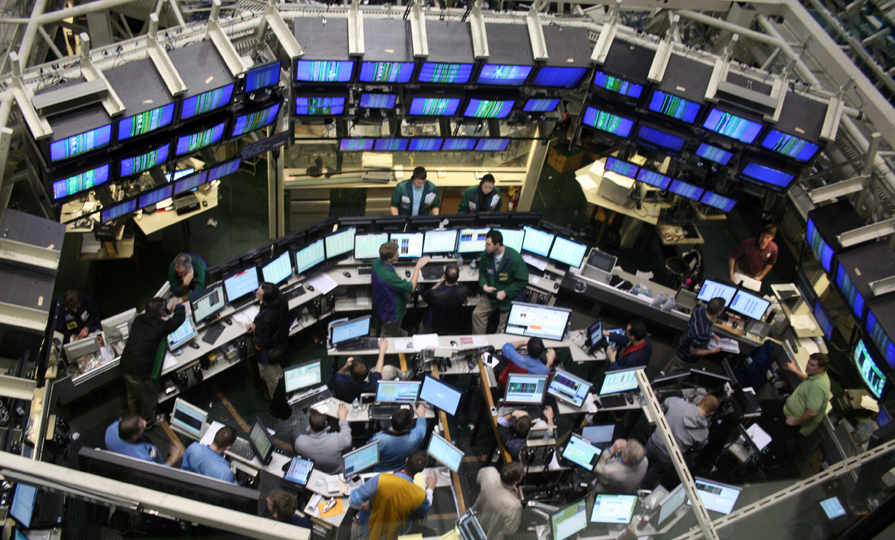
\includegraphics[scale=.25]{cboe}
\end{center}
\end{figure}
\end{frame}

% Option Basics
\begin{frame}{Option Basics}
\begin{itemize}
\item A \textit{financial option} is a contract that gives its owner the \underline{right} (but not the \underline{obligation}) to purchase or sell an asset at a fixed price at some future date. 
\item There are two kinds of options:
\begin{itemize}
\item a \textit{call option} gives the owner the right to \underline{buy} the asset;
\item a \textit{put option} gives the owner the right to \underline{sell} the asset. 
\end{itemize}
\item For every owner, there is a \textit{option writer}. 
\item Disney trades for \$95.72. 
\item You can buy the option to \underline{buy} Disney for \$90.00 on or before Jul. 1, for \$10.00.
\item You can buy the option to \underline{sell} Disney for \$90.00 on or before Jul. 1 for \$0.24.  
\end{itemize}
\end{frame}

% Understanding Option Contracts
\begin{frame}{Understanding Option Contracts}
\begin{itemize}
\item When the owner buys or sells a share of stock at the agreed-upon price, she is \textit{exercising} the option. 
\item The price at which the holder buys or sells the shares of stock when the option is exercised is called the \textit{strike price}. 
\item There are two (more) kinds of options:
\begin{itemize}
\item American options allow their holders to exercise the option on any date up to and including the \textit{expiration date};
\item European options allow their holders to exercise the option only on the expiration date. 
\end{itemize}
\item Option owners are said to be \textit{long} and option writers are said to be \textit{short}. 
\end{itemize}
\end{frame}

% Understanding Option Contracts
\begin{frame}{Understanding Option Contracts}
\begin{itemize}
\item Options are not free. 
\item When you sell an option, you get paid for it. 
\item The market price of the option is also called the \textit{option premium}. 
\end{itemize}
\end{frame}

% Interpreting Stock Option Quotations
\begin{frame}{Interpreting Stock Option Quotations}
\begin{itemize}
\item Stock options are traded on organized exchanges. 
\item The oldest and largest is the Chicago Board Options Exchange (CBOE). 
\item By convention, all traded options expire on the Saturday following the third Friday of the month. 
\item Stock option contracts are always written on 100 shares of stock. 
\item More vocabulary: an option is said to be
\begin{itemize}
\item \textbf{in-the-money} if the payoff from exercising an option immediately is positive;
\item \textbf{at-the-money} if the exercise price equals the current price of the stock;
\item \textbf{out-of-the-money} if the payoff from exercising an option immediately is negative;
\end{itemize}
\item The terms deep-in-the-money are commonly used deep-out-of-the-money.
\end{itemize}
\end{frame}

% Options on Other Financial Securities
\begin{frame}{Options on Other Financial Securities}
\begin{itemize}
\item There are options on the S\&P 500, the DIJA, etc. 
\item Index puts allow investors to protect themselves against market downturns. 
\item If you use an option to reduce risk, you are said to \textit{hedge}.
\item If you use an option to bet on market movements, you are said to \textit{speculate}.
\end{itemize}
\begin{figure}[H]
\begin{center}

\includegraphics[scale=.25]{options}
\end{center}
\end{figure}
\end{frame}

% Long Position in a Call
\begin{frame}{Long Position in a Call}
Let $S$ denote the stock price at expiration, $K$ the strike price, and $C$ the value of the call option. The value of a \textbf{long position} in the \textbf{call option} at expiration is 
\begin{equation*}
\text{Value of Long Call}=C=\max\{S-K,0\}. 
\end{equation*}
\begin{figure}[H]
\begin{center}

\includegraphics[scale=.4]{longcall}
\end{center}
\end{figure}
\end{frame}

\begin{frame}{Examples: Long Call}
You purchase one MBI July 120 call contract (equaling 100 shares) for a premium of \$5. You hold the option until the expiration date, when MBI stock sells for \$123 per share. What is your profit/loss? \\
\vspace{.5in}
\pause
Long call profit = $\max$\{0, (\$123 - \$120)(100)\} - \$500 = -\$200
\end{frame}

% Long Position in a Put
\begin{frame}{Long Position in a Put}
Let $S$ denote the stock price at expiration, $K$ the strike price, and $P$ the value of the put option. The value of a \textbf{long position} in the \textbf{put option} at expiration is 
\begin{equation*}
\text{Value of Long Put}=P=\max\{K-S,0\}. 
\end{equation*}
\begin{figure}[H]
\begin{center}
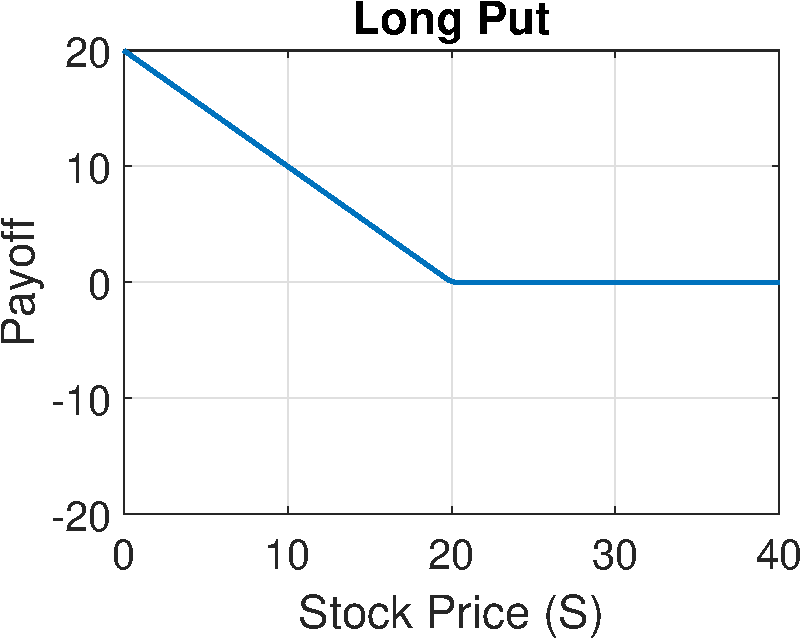
\includegraphics[scale=.4]{longput}
\end{center}
\end{figure}
\end{frame}


\begin{frame}{Examples: Long Put}
You purchase one MBI July 120 put contract (equaling 100 shares) for a premium of \$3. You hold the option until the expiration date, when MBI stock sells for \$123 per share. What is your profit/loss?\\
\vspace{.5in}
\pause
Long put profit = $\max$\{0, (\$120 - \$123)(100)\} - \$300 = -\$300
\end{frame}

% Short Position in a Call
\begin{frame}{Short Position in a Call}
Let $S$ denote the stock price at expiration, $K$ the strike price, and $C$ the value of the call option. The value of a \textbf{short position} in the \textbf{call option} at expiration is 
\begin{equation*}
\text{Value of Short Call}=-C=-\max\{S-K,0\}. 
\end{equation*}
\begin{figure}[H]
\begin{center}
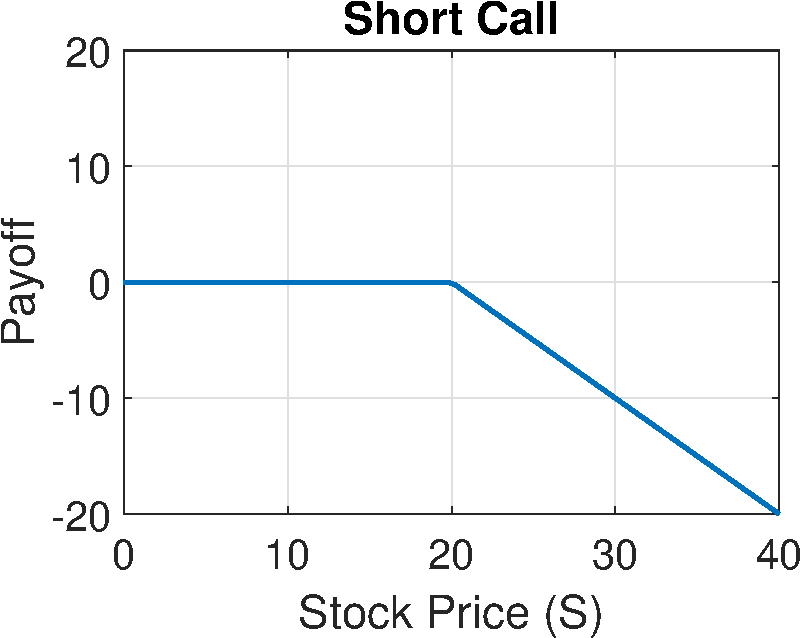
\includegraphics[scale=.4]{shortcall}
\end{center}
\end{figure}
\end{frame}

\begin{frame}{Examples: Short Call}
You write one MBI July 120 call contract (equaling 100 shares) for a premium of \$4. You hold the option until the expiration date, when MBI stock sells for \$121 per share. What is your profit/loss?\\
\vspace{.5in}
\pause
Short call profit = $\min$\{0, (\$120 - \$121)(100)\} + \$400 = \$300
\end{frame}

% Short Position in a Put
\begin{frame}{Short Position in a Put}
Let $S$ denote the stock price at expiration, $K$ the strike price, and $P$ the value of the put option. The value of a \textbf{short position} in the \textbf{put option} at expiration is 
\begin{equation*}
\text{Value of Short Put}=-P=-\max\{K-S,0\}. 
\end{equation*}
\begin{figure}[H]
\begin{center}
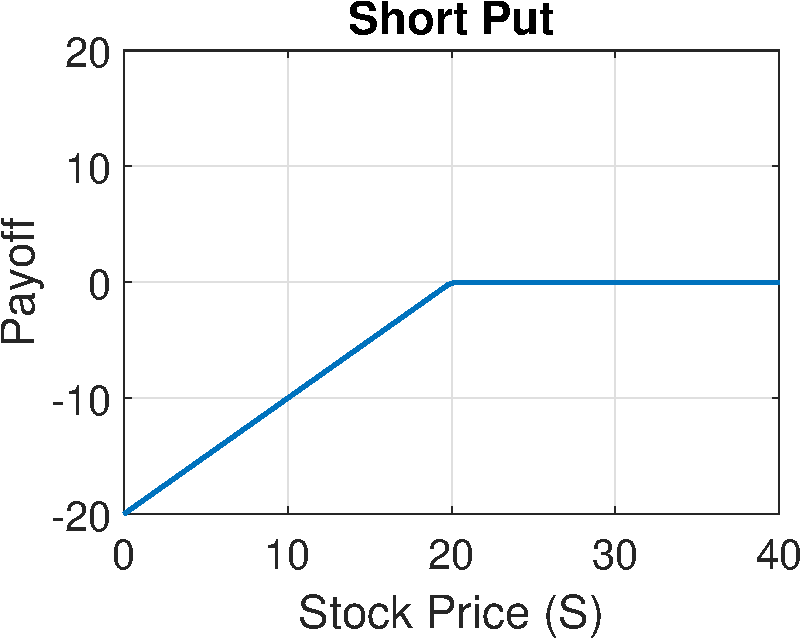
\includegraphics[scale=.4]{shortput}
\end{center}
\end{figure}
\end{frame}

% The Straddle
\begin{frame}{The Straddle}
Let $S$ denote the stock price at expiration, $K$ the strike price, $C$ the value of the call option, and $P$ the value of the put option. A \textbf{straddle} is \textbf{long} a \textbf{call} and \textbf{long} a \text{put} with the same strike. Its value at expiration is 
\begin{equation*}
\text{Value of Straddle}=C(S;K)+P(S;K)=\max\{S-K,K-S\}. 
\end{equation*}
\begin{figure}[H]
\begin{center}
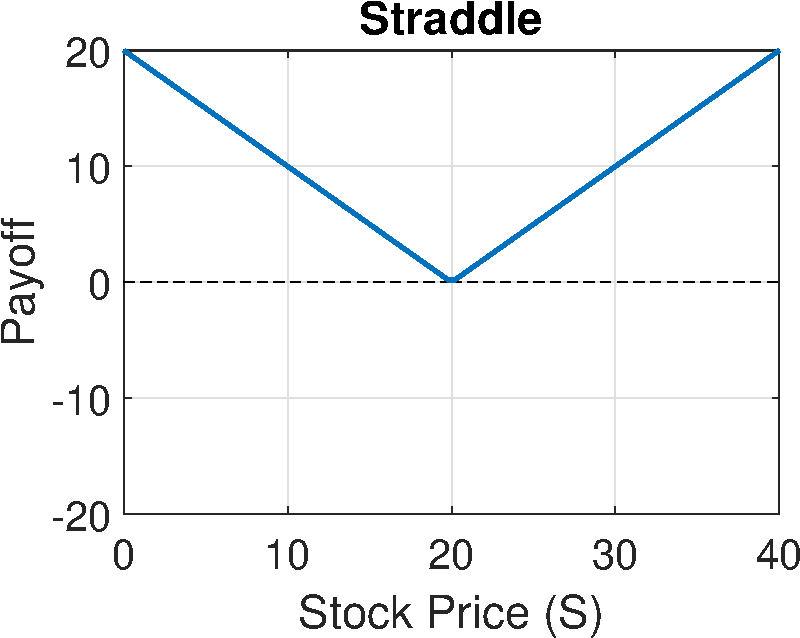
\includegraphics[scale=.4]{straddle}
\end{center}
\end{figure}
\end{frame}

% The Butterfly
\begin{frame}{The Butterfly}
Let $S$ denote the stock price at expiration, $K_{L}<K_{M}<K_{H}$  strike prices, and $C$ the value of the call option. A \textbf{butterfly} is \textbf{long} a  \textbf{call} with a \textbf{low strike}, \textbf{long} a \textbf{call} with a \textbf{high strike}, and \textbf{short} two \textbf{calls} with \textbf{medium strikes}. Its value at expiration is
\begin{equation*}
\text{Value of Butterfly}=C(S;K_{H})+C(S;K_{L})-2C(S;K_{M}). 
\end{equation*}
\begin{figure}[H]
\begin{center}
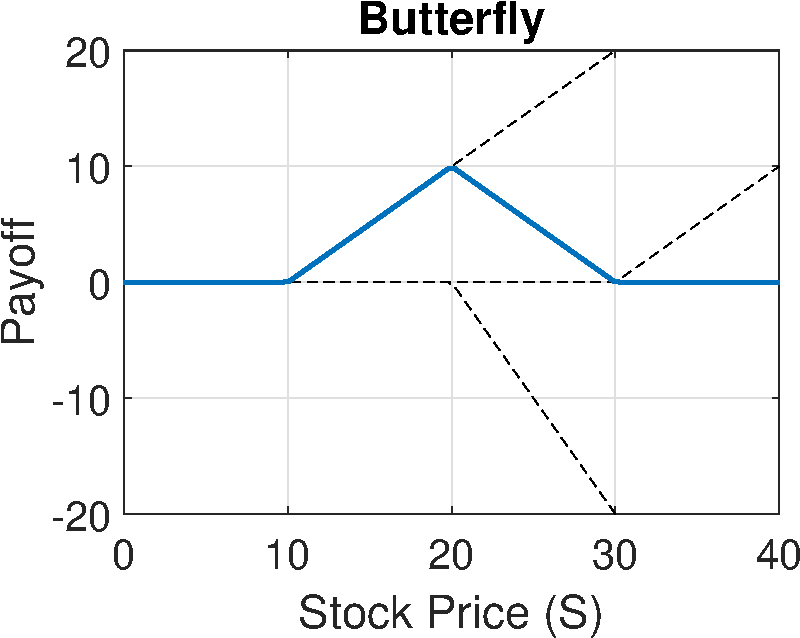
\includegraphics[scale=.4]{butterfly}
\end{center}
\end{figure}
\end{frame}

% The Covered Call
\begin{frame}{The Covered Call}
Let $S$ denote the stock price at expiration, $K$ the strike price, and $C$ the value of the call option. A \textbf{covered call} is \textbf{long} the \textbf{underlying} and \textbf{short} a \textbf{call}. Its value at expiration is
\begin{equation*}
\text{Value of Covered Call}=S-C(S;K)=\min\{S,K\}
\end{equation*}
\begin{figure}[H]
\begin{center}
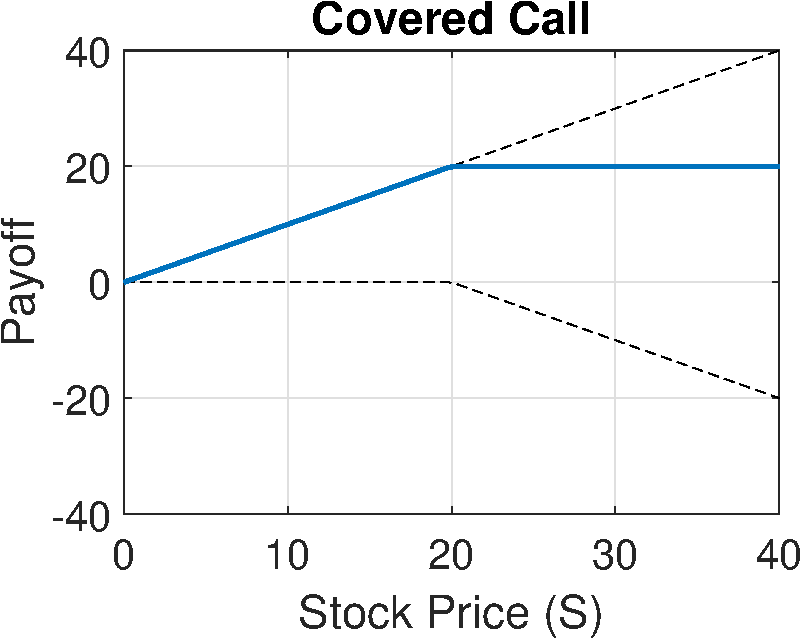
\includegraphics[scale=.4]{coveredcall}
\end{center}
\end{figure}
\end{frame}

% The Married Put
\begin{frame}{The Married Put}
Let $S$ denote the stock price at expiration, $K$ the strike price, and $P$ the value of the put option. A \textbf{married put} is \textbf{long} the \textbf{underlying} and \textbf{long} a \textbf{put}. Its value at expiration is
\begin{equation*}
\text{Value of Married Put}=S+P(S;K)=\max\{K,S\}.  
\end{equation*}
\begin{figure}[H]
\begin{center}
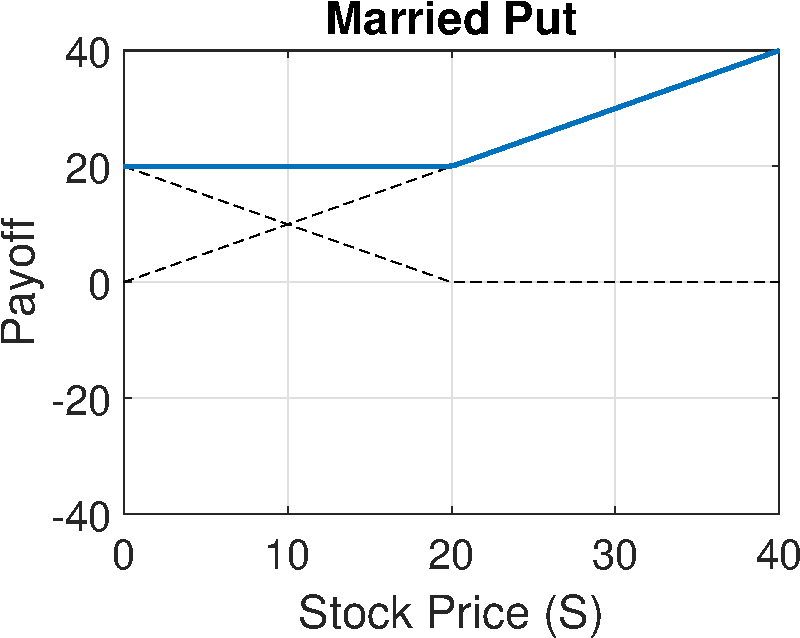
\includegraphics[scale=.4]{marriedput}
\end{center}
\end{figure}
\end{frame}

% The Structured Product
\begin{frame}{The Structured Product}
The Minions' structured product was \textbf{long} the \textbf{risk-free asset} and \textbf{long} a \textbf{call}. Its value at expiration was
\begin{equation*}
\text{Value of Structured Product}=K+C(S;K)=\max\{S,K\}.  
\end{equation*}
\begin{figure}[H]
\begin{center}
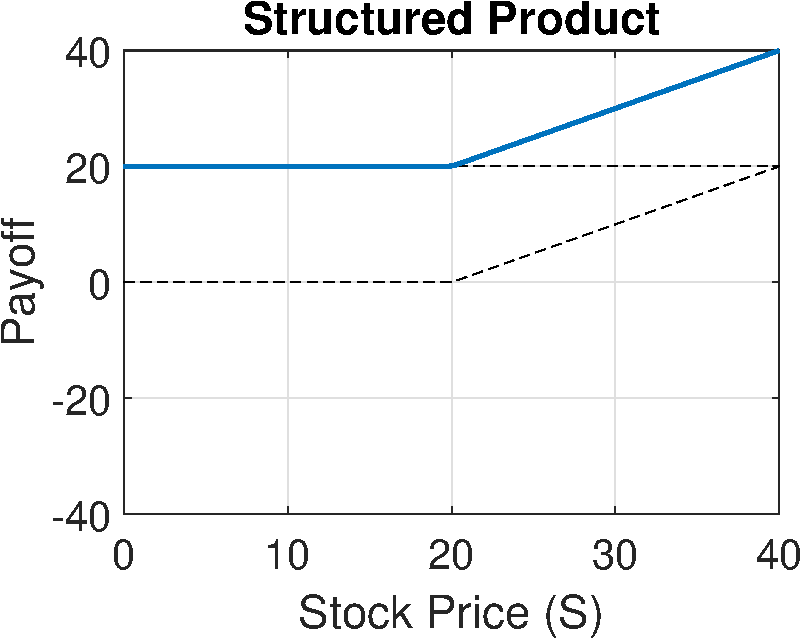
\includegraphics[scale=.4]{structuredproduct}
\end{center}
\end{figure}
\end{frame}

% Put-Call Parity
\begin{frame}{Put-Call Parity}
\begin{itemize}
\item Hmmm...the Structured Product  has the same payoff as the Married Put. 
\item Two securities with the same cash flows must have the same price. 
\item \textbf{Put-Call Parity} says that
\begin{equation*}
\overbrace{S+P}^{\text{Married Put}}=\overbrace{PV(K)+C}^{\text{Structured Product}}
\end{equation*}
\item Put-call parity gives the price of a call in terms of the price of a put, the underlying stock, and a zero-coupon bond. 
\end{itemize}
\end{frame}

% Factors Affecting Option Prices
\begin{frame}{Factors Affecting Option Prices}
\begin{itemize}
\item \textbf{Strike Price and Stock Price:} the value of a call is \underline{decreasing} in the strike price (the higher the strike, the lower the value); the value of a call is \underline{increasing} in the price of the stock (the higher the price of the stock, the higher the value). 
\item \textbf{Arbitrage Bounds on Option Prices:} 
\begin{itemize}
\item an American option carries all of the same rights and privileges as an otherwise equivalent European option. The American option can't be worth less. 
\item a put option can't be worth more than its strike price and a call can't be worth more than the stock itself.
\end{itemize}
\end{itemize}
\end{frame}

% Factors Affecting Option Prices
\begin{frame}{Factors Affecting Option Prices}
\begin{itemize}
\item \textbf{Option Prices and the Exercise Date:} 
\begin{itemize}
\item (for American options,) the longer the time to the exercise date, the more valuable the option.
\item An American option with a later exercise date cannot be worth less than an otherwise identical American option with an earlier exercise date.
\item These arguments \underline{do not} carry through for European options.
\end{itemize}
\item \textbf{Option Prices and Volatility:} 
\begin{itemize}
\item The value of an option generally increases with the volatility of the stock.
\item Increasing the volatility of the stock increases the likelihood that the stock will take on extreme values (which is where options are valuable).
\end{itemize}
\end{itemize}
\end{frame}

% Equity as a Call Option
\begin{frame}{Equity as a Call Option}
Consider a firm with \$10m in debt. It will only operate for one year. At the end of the year, its assets maybe worth anywhere from \$0m to \$40m. What's the payoff to \textbf{equityholders}?
\begin{equation*}
E=\max\{A-K,0\}\overset{!}{=}\max\{A-\$10m,0\}. 
\end{equation*}
\begin{figure}[H]
\begin{center}

\includegraphics[scale=.4]{equity}
\end{center}
\end{figure}
\end{frame}

% Debt as a Covered Call
\begin{frame}{Debt as a Covered Call}
Consider a firm with \$10m in debt. It will only operate for one year. At the end of the year, its assets maybe worth anywhere from \$0m to \$40m. What's the payoff to \textbf{debtholders}?
\begin{equation*}
D=\min\{A,K\}\overset{!}{=}\min\{A,\$10m\}. 
\end{equation*}
\begin{figure}[H]
\begin{center}
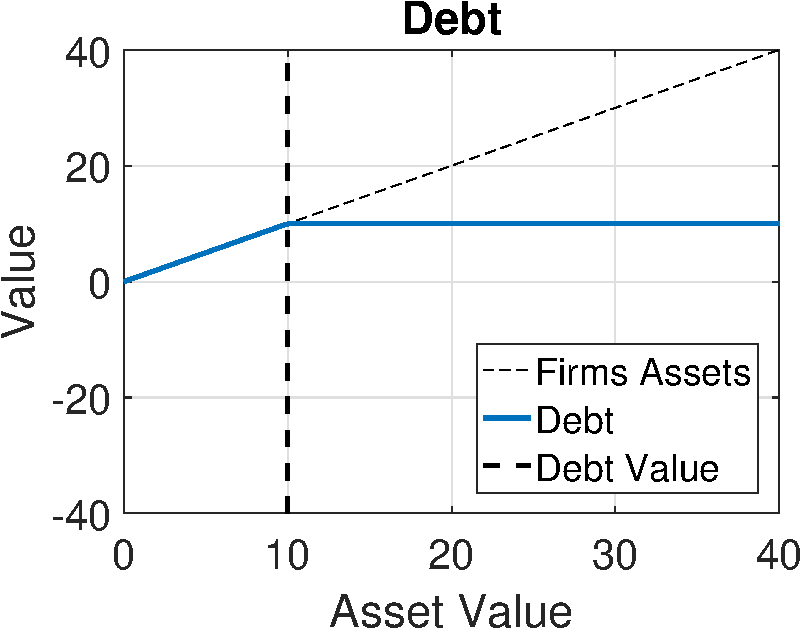
\includegraphics[scale=.4]{debt}
\end{center}
\end{figure}
\end{frame}

% The Total Payoff
\begin{frame}{The Total Payoff}
Now what's the \textbf{total payoff}?
\begin{equation*}
E+D=\max\{A-K,0\}+\min\{A,K\}=A
\end{equation*}
\begin{figure}[H]
\begin{center}
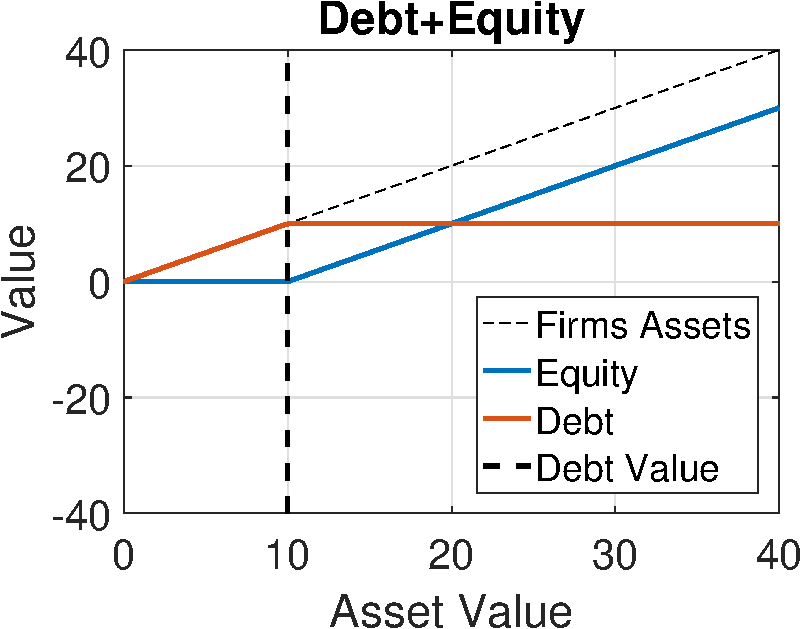
\includegraphics[scale=.4]{debtequity}
\end{center}
\end{figure}
\end{frame}

% The Total Payoff
\begin{frame}{The Total Payoff}
Now what's the \textbf{total payoff}?
\begin{equation*}
E+D=\max\{A-K,0\}+\min\{A,K\}=A
\end{equation*}
\begin{figure}[H]
\begin{center}
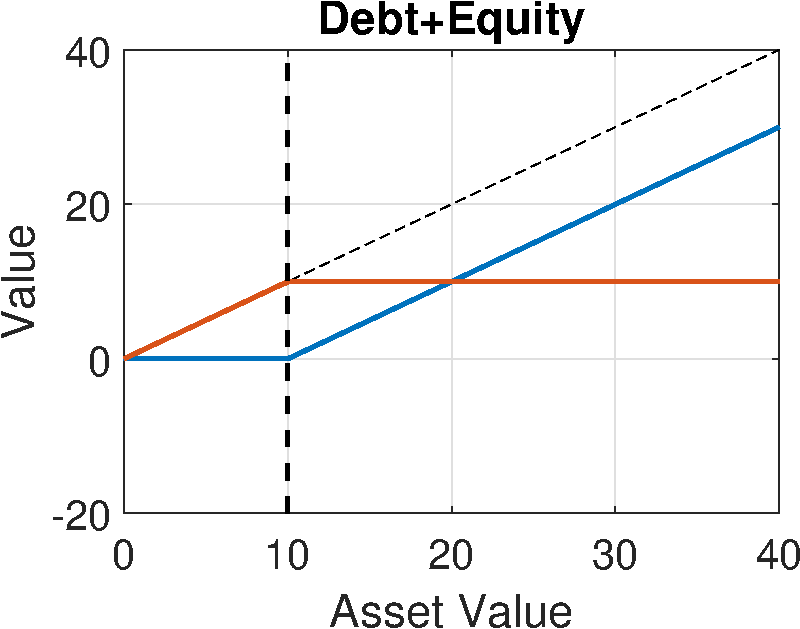
\includegraphics[scale=.4]{debtequity2}
\end{center}
\end{figure}
\end{frame}

% Modigliani Miller Redeux
\begin{frame}{Modigliani Miller}
\begin{itemize}
\item \textbf{Option-Speak:} a call plus a covered call equals the underlying stock
\begin{equation*}
C+(S-C)=S
\end{equation*}
\textbf{\color{magenta}{
regardless of the strike price}}.
\item \textbf{Capital-Structure-Speak:} equity plus debt equals the underlying cash flows
\begin{equation*}
E_{L}+D_{L}=V
\end{equation*}
\textbf{\color{magenta}{
regardless of the amount of debt}}.
\item Options provide us with an elegant proof of the Modigliani Miller Theorem, which says that the exact mix of debt and equity does not affect firm value.
\end{itemize}
\end{frame}

\end{document}
